\section{Applicazioni}

\subsection{Modello readers and writers}
Il modello readers and writers rappresenta un sistema concorrente in cui $N$
processi accedono ad una risorsa condivisa in lettura o scrittura. La lettura è
shared, la scrittura exclusive.  In figura \ref{petri2} è  mostrata la rete di
petri che lo implementa.

\begin{figure}[!hb]
	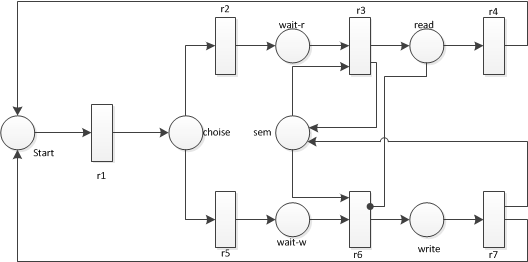
\includegraphics[width=10cm]{../resources/images/petri2.png}
	\label{petri2}
	\caption{Rete di petri simulata da CTMC-READER\_WRITER}
\end{figure}

Il modello si può esprimere in modo stocastico, facendo dipendere dal numero di
token i rate da un place all'altro. Implementativamente, per rapprentare gli
stati si utilizza un set di variabili, una per place, che hanno come valore il
numero di token.
\begin{Verbatim}[fontsize=\small]
var VL : VarList .
var N, M : Nat .

*** Start
crl [model] : < v("start" , N) v("choose" , M) VL > =>
             [10.0 * float(N)]
               < v("start" , N + -1) v("choose" , M + 1) VL >
             if N > 0 .
*** Read
crl [model] : < v("choose" , N) v("waitr" , M) VL > =>
             [5.0 * float(N)]
               < v("choose" , N + -1) v("waitr" , M + 1) VL >
             if N > 0 .
crl [model] : < v("waitr" , N) v("read" , M) v("sem" , 1) VL > =>
             [20.0 * float(N)]
               < v("waitr" , N + -1) v("read" , M + 1) v("sem" , 1) VL >
             if N > 0 .
crl [model] : < v("read" , N) v("start" , M) VL > =>
             [50.0 * float(N)]
               < v("read" , N + -1) v("start" , M + 1) VL >
             if N > 0 .
*** Write
crl [model] : < v("choose" , N) v("waitw" , M) VL > =>
             [5.0 * float(N)]
               < v("choose" , N + -1) v("waitw" , M + 1) VL >
             if N > 0 .
crl [model] : < v("waitw" , N) v("write" , M) v("sem" , 1)
                                            v("read" , 0) VL > =>
             [40.0 * float(N)]
               < v("waitw" , N + -1) v("write" , M + 1)
                                               v("sem" , 0) v("read" ,0) VL >
             
             if N > 0 .
crl [model] : < v("write" , N) v("start" , M) v("sem" , 0) VL > =>
             [50.0 * float(N)]
               < v("write" , N + -1) v("start" , M + 1) v("sem" , 1) VL >
             if N > 0 .

\end{Verbatim}
L'overview è gestita stampando a video informazioni come il numero di read, di
write e il tempo intercorso dall'ultima overview.

\begin{verbatim}
	rl [overwiew] : [El] => print(El) .

	ceq print(T1 : S1 - El - T2 : S2) = [T2 : S2]
		if 	T3 := T2 - T1 /\ nc(NR,NW) := numRW(T1 : S1 - El - T2 : S2)
		[ print "In " T3 " sec\n\tFrom " T1 " to " T2 "\n\tNumReads: " NR "\n\tNumWrites: " NW ] .

	ceq numRW(T1 : < v("read" , N1) > < v("write" , M1) > S1 - T2 :
	< v("read" , N2) > < v("write" , M2) > S2 - El) = nc(N + NR, M + NW)
	if	N := ( if N2 > N1 then 1 else 0 fi ) /\
	M := ( if M2 > M1 then 1 else 0 fi )/\
	nc(NR, NW) := numRW(T2 : < v("read" , N2) > < v("write" , M2) > - El) .
	
	eq numRW(El) = nc(0, 0) [ owise ] .
\end{verbatim}

\subsection{Modello M/M/C/K per la simulazione delle code}

M/M/C/K è un modello utilizzato nella teoria delle code per analizzare e
simulare il comportamento di un sistema di $C$ server che elaborano un task
alla volta. I task nascono con un certo rate $\tau$ e sono memorizzati in un
buffer di dimensione $K$. Se il buffer è pieno sono perduti. I task muoiono
(sono svolti dai server) con un rate che vale $\mu * N$, dove N è il numero dei
task, se $N \leq C$, altrimenti il rate vale $\mu * C$.

Gli stati del modello sono enumerabili da un numero naturale, tuttavia nel
modello sono inclusi anche altri elementi di configurazione ed utilità come la
dimensione del buffer, il numero di server e il numero di task perduti.

\begin{Verbatim}[fontsize=\small]
var N K L C : Nat .
var VL : VarList .

*** Accodamento nel Buffer
crl [model] : < v("buffersize" , K) v("buffer", N) VL > =>
              [ 0.535 ] < v("buffersize" , K) v("buffer", N + 1) VL >
              if N < K .
*** Buffer pieno
crl [model] : < v("buffersize" , K) v("buffer", N) v("losts", L) VL > =>
              [ 0.535 ] < v("buffersize" , K) v("buffer", N)
                                               v("losts", L + 1) VL >
              if N >= K .
*** Svolgimento di task (caso N < C)
crl [model] : < v("nserver" , C) v("buffer", N) VL > =>
              [0.120 * float(N)] < v("buffer", N + -1) v("nserver" , C) VL >
              if N > 0 /\ N < C .
*** Svolgimento di task (caso N >= C)
crl [model] : < v("nserver" , C) v("buffer", N) VL > =>
              [0.120 * float(C)] < v("buffer", N + -1) v("nserver" , C) VL >
              if N > 0 /\ N >= C .

\end{Verbatim}

\subsection{Modello di test della Bromosulftaleina}

\begin{figure}[!ht]
	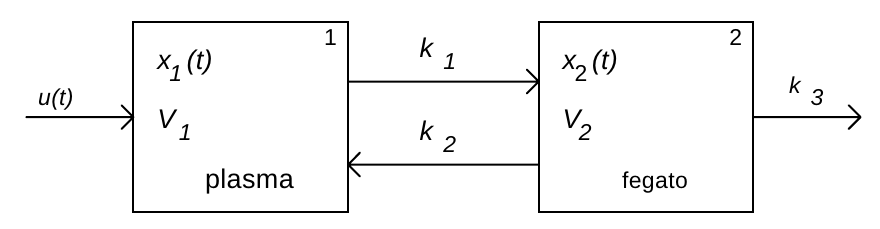
\includegraphics[width=10cm]{../resources/images/BSF.png}
	\label{bsf}
	\caption{Modello BSF (\cite{gnudi})}
\end{figure}

Il test BSF \cite{gnudi} è semplificabile considerandolo un sistema a due compartimenti
(uno per il fegato, l'altro per il plasma), con un certo rate di trasferimento. Si
suppone un inserimento del colorante nel plasma istantaneo e si può
semplificarlo imponendo la condizione inziale del plasma pari alla quantità di
colorante iniettato. Il colorante, quando entra nel fegato, scompare con un
certo rate e è riassorbito nel plasma con un altro rate. Per completezza si
considera anche il volume dei due compartimenti (vedi figura \ref{bsf}).

Il modello è semplificato al caso di trasferimenti di colorante discreti.

\begin{verbatim}
var N K L : Nat .
var VP VF : Nat .
var VL : VarList .
	
	
*** Passaggio colorante dal compartimento plasma a fegato
crl [model] : < v("volplasma", VP) v("volfegato", VF)
                       v("plasma", N) v("fegato", L) > =>
              [ 0.454 * float(N) / float(VP) ]
              < v("volplasma", VP) v("volfegato", VF)
                v("plasma", N + -1)  v("fegato", L + 1) >
              if N > 0 /\ L < VF .

*** Passaggio colorante dal compartimento fegato a plasma            
crl [model] : < v("volfegato", VF) v("volplasma", VP)
                       v("plasma", N) v("fegato", L) > =>
             [ 0.698 * float(L) / float(VF) ]
             < v("volfegato", VF) v("volplasma", VP)
               v("plasma", N + 1) v("fegato", L + -1) >
             if L > 0 /\ N < VP .
		
*** Scomparsa del colorante dal compartimento fegato
crl [model] : < v("volfegato", VF) v("fegato", L) VL > =>
             [ 0.432 * float(L) / float(VF) ]
             < v("volfegato", VF) v("fegato", L + -1) VL >
             if L > 0 .
	
\end{verbatim}

Per un numero di step tendente all'infinito, prima o poi il modello entrerà in
deadlock.










